% !TeX spellcheck = hu_HU
% !TeX encoding = UTF-8
% !TeX program = xelatex
% TODO Change language to en_GB (recommended) or en_US for English documents
\documentclass[11pt,a4paper,oneside]{report}             % Single-side
%\documentclass[11pt,a4paper,twoside,openright]{report}  % Duplex

% thanks to http://tex.stackexchange.com/a/47579/71109
\usepackage{ifxetex}
\usepackage{ifluatex}
\newif\ifxetexorluatex % a new conditional starts as false
\ifnum 0\ifxetex 1\fi\ifluatex 1\fi>0
   \xetexorluatextrue
\fi

\ifxetexorluatex
  \usepackage{fontspec}
\else
  \usepackage[T1]{fontenc}
  \usepackage[utf8]{inputenc}
  \usepackage[lighttt]{lmodern}
  \ttfamily\DeclareFontShape{T1}{lmtt}{m}{it}{<->sub*lmtt/m/sl}{}
\fi

\usepackage[english,magyar]{babel} % Alapértelmezés szerint utoljára definiált nyelv lesz aktív, de később külön beállítjuk az aktív nyelvet.

\usepackage{emptypage} % omit page number on empty pages

%\usepackage{cmap}
\usepackage{amsfonts,amsmath,amssymb} % Mathematical symbols.
%\usepackage[ruled,boxed,resetcount,linesnumbered]{algorithm2e} % For pseudocodes. % beware: this is not compatible with LuaLaTeX, see http://tex.stackexchange.com/questions/34814/lualatex-and-algorithm2e
\usepackage{booktabs} % For publication quality tables for LaTeX
\usepackage{graphicx}

%\usepackage{fancyhdr}
%\usepackage{lastpage}

\usepackage{anysize}
%\usepackage{sectsty}
\usepackage{setspace} % For setting line spacing

\usepackage[unicode]{hyperref} % For hyperlinks in the generated document.
\usepackage{xcolor}
\usepackage{listings} % For source code snippets.

\usepackage[amsmath,thmmarks]{ntheorem} % Theorem-like environments.

\usepackage[hang]{caption}

\usepackage{subfigure}

\singlespacing

\newcommand{\selecthungarian}{
	\selectlanguage{magyar}
	\setlength{\parindent}{2em}
	\setlength{\parskip}{0em}
	\frenchspacing
}

\newcommand{\selectenglish}{
	\selectlanguage{english}
	\setlength{\parindent}{0em}
	\setlength{\parskip}{0.5em}
	\nonfrenchspacing
	\renewcommand{\figureautorefname}{Figure}
	\renewcommand{\tableautorefname}{Table}
	\renewcommand{\partautorefname}{Part}
	\renewcommand{\chapterautorefname}{Chapter}
	\renewcommand{\sectionautorefname}{Section}
	\renewcommand{\subsectionautorefname}{Section}
	\renewcommand{\subsubsectionautorefname}{Section}
}

\usepackage[numbers]{natbib}
\usepackage{xspace}


%TODO Set the main variables
\newcommand{\vikszerzoVezeteknev}{Gáti}
\newcommand{\vikszerzoKeresztnev}{László Dávid}

\newcommand{\vikkonzulensAMegszolitas}{}
\newcommand{\vikkonzulensAVezeteknev}{Farkas}
\newcommand{\vikkonzulensAKeresztnev}{Rebeka}

\newcommand{\vikkonzulensBMegszolitas}{}
\newcommand{\vikkonzulensBVezeteknev}{}
\newcommand{\vikkonzulensBKeresztnev}{}

\newcommand{\vikkonzulensCMegszolitas}{}
\newcommand{\vikkonzulensCVezeteknev}{}
\newcommand{\vikkonzulensCKeresztnev}{}

\newcommand{\vikcim}{MagicDraw plugin továbbfejlesztése} % Cím
\newcommand{\viktanszek}{\bmemit} % Tanszék
\newcommand{\vikdoktipus}{\msconlabi} % Dokumentum típusa (\bsc vagy \msc)
\newcommand{\vikmunkatipusat}{Önlab 1} % a "hallgató nyilatkozat" részhez: szakdolgozatot vagy diplomatervet

\input{include/tdk-variables}
\newcommand{\szerzoMeta}{\vikszerzoVezeteknev{} \vikszerzoKeresztnev} % egy szerző esetén
%\newcommand{\szerzoMeta}{\vikszerzoVezeteknev{} \vikszerzoKeresztnev, \tdkszerzoB} % két szerző esetén

%TODO Language configuration -- choose one
% Beállítások magyar nyelvű dolgozathoz
%%--------------------------------------------------------------------------------------
% Elnevezések
%--------------------------------------------------------------------------------------
\newcommand{\bme}{Budapesti Műszaki és Gazdaságtudományi Egyetem}
\newcommand{\vik}{Villamosmérnöki és Informatikai Kar}

\newcommand{\bmemit}{Méréstechnika és Információs Rendszerek Tanszék}

\newcommand{\keszitette}{Készítette}
\newcommand{\konzulens}{Konzulens}

\newcommand{\bsc}{Szakdolgozat}
\newcommand{\msc}{Diplomaterv}
\newcommand{\tdk}{TDK dolgozat}
\newcommand{\bsconlab}{BSc Önálló laboratórium}
\newcommand{\msconlabi}{MSc Önálló laboratórium 1.}
\newcommand{\msconlabii}{MSc Önálló laboratórium 2.}

\newcommand{\pelda}{Példa}
\newcommand{\definicio}{Definíció}
\newcommand{\tetel}{Tétel}

\newcommand{\bevezetes}{Bevezetés}
\newcommand{\koszonetnyilvanitas}{Köszönetnyilvánítás}
\newcommand{\fuggelek}{Függelék}
\newcommand{\uppaal}{UPPAAL}

% Opcionálisan átnevezhető címek
%\addto\captionsmagyar{%
%\renewcommand{\listfigurename}{Saját ábrajegyzék cím}
%\renewcommand{\listtablename}{Saját táblázatjegyzék cím}
%\renewcommand{\bibname}{Saját irodalomjegyzék név}
%}

\newcommand{\szerzo}{\vikszerzoVezeteknev{} \vikszerzoKeresztnev}
\newcommand{\vikkonzulensA}{\vikkonzulensAMegszolitas\vikkonzulensAVezeteknev{} \vikkonzulensAKeresztnev}
\newcommand{\vikkonzulensB}{\vikkonzulensBMegszolitas\vikkonzulensBVezeteknev{} \vikkonzulensBKeresztnev}
\newcommand{\vikkonzulensC}{\vikkonzulensCMegszolitas\vikkonzulensCVezeteknev{} \vikkonzulensCKeresztnev}

\newcommand{\selectthesislanguage}{\selecthungarian}

\bibliographystyle{huplain}

\def\lstlistingname{lista}

\newcommand{\appendixnumber}{6}  % a fofejezet-szamlalo az angol ABC 6. betuje (F) lesz

% Settings for English documents
%--------------------------------------------------------------------------------------
% Elnevezések
%--------------------------------------------------------------------------------------
\newcommand{\bme}{Budapesti Műszaki és Gazdaságtudományi Egyetem}
\newcommand{\vik}{Villamosmérnöki és Informatikai Kar}

\newcommand{\bmemit}{Méréstechnika és Információs Rendszerek Tanszék}

\newcommand{\keszitette}{Készítette}
\newcommand{\konzulens}{Konzulens}

\newcommand{\bsc}{Szakdolgozat}
\newcommand{\msc}{Diplomaterv}
\newcommand{\tdk}{TDK dolgozat}
\newcommand{\bsconlab}{BSc Önálló laboratórium}
\newcommand{\msconlabi}{MSc Önálló laboratórium 1.}
\newcommand{\msconlabii}{MSc Önálló laboratórium 2.}

\newcommand{\pelda}{Példa}
\newcommand{\definicio}{Definíció}
\newcommand{\tetel}{Tétel}

\newcommand{\bevezetes}{Bevezetés}
\newcommand{\koszonetnyilvanitas}{Köszönetnyilvánítás}
\newcommand{\fuggelek}{Függelék}
\newcommand{\uppaal}{UPPAAL}

% Opcionálisan átnevezhető címek
%\addto\captionsmagyar{%
%\renewcommand{\listfigurename}{Saját ábrajegyzék cím}
%\renewcommand{\listtablename}{Saját táblázatjegyzék cím}
%\renewcommand{\bibname}{Saját irodalomjegyzék név}
%}

\newcommand{\szerzo}{\vikszerzoVezeteknev{} \vikszerzoKeresztnev}
\newcommand{\vikkonzulensA}{\vikkonzulensAMegszolitas\vikkonzulensAVezeteknev{} \vikkonzulensAKeresztnev}
\newcommand{\vikkonzulensB}{\vikkonzulensBMegszolitas\vikkonzulensBVezeteknev{} \vikkonzulensBKeresztnev}
\newcommand{\vikkonzulensC}{\vikkonzulensCMegszolitas\vikkonzulensCVezeteknev{} \vikkonzulensCKeresztnev}

\newcommand{\selectthesislanguage}{\selecthungarian}

\bibliographystyle{huplain}

\def\lstlistingname{lista}

\newcommand{\appendixnumber}{6}  % a fofejezet-szamlalo az angol ABC 6. betuje (F) lesz


\input{include/preamble}

%--------------------------------------------------------------------------------------
% Table of contents and the main text
%--------------------------------------------------------------------------------------
\begin{document}

%TODO These define guidelines -- remove these
%~~~~~~~~~~~~~~~~~~~~~~~~~~~~~~~~~~~~~~~~~~~~~~~~~~~~~~~~~~~~~~~~~~~~~~~~~~~~~~~~~~~~~~


\selectthesislanguage

%TODO Titlepage -- choose one from below
%~~~~~~~~~~~~~~~~~~~~~~~~~~~~~~~~~~~~~~~~~~~~~~~~~~~~~~~~~~~~~~~~~~~~~~~~~~~~~~~~~~~~~~
\include{include/titlepage}		   % Szakdolgozat/Diplomaterv címlap
%\include{include/titlepage-tdk}	% TDK címlap
%\include{include/titlepage-otdk}   % OTDK címlap


% Table of Contents
%~~~~~~~~~~~~~~~~~~~~~~~~~~~~~~~~~~~~~~~~~~~~~~~~~~~~~~~~~~~~~~~~~~~~~~~~~~~~~~~~~~~~~~
\tableofcontents\vfill


% Declaration and Abstract
%~~~~~~~~~~~~~~~~~~~~~~~~~~~~~~~~~~~~~~~~~~~~~~~~~~~~~~~~~~~~~~~~~~~~~~~~~~~~~~~~~~~~~~


% The main part of the thesis
%~~~~~~~~~~~~~~~~~~~~~~~~~~~~~~~~~~~~~~~~~~~~~~~~~~~~~~~~~~~~~~~~~~~~~~~~~~~~~~~~~~~~~~
\pagenumbering{arabic}

%TODO import your own content
%----------------------------------------------------------------------------
\chapter{\bevezetes}
%----------------------------------------------------------------------------

A IT technológiák térnyerésével egyre több és komplexebb rendszer készül, melyeknek sokszor valós időben kell működni. Mivel ilyen rendszerek jellemzően valamilyen biztonság kritikus környezetben működnek, elengedhetetlené válik ezek gondos megtervezése és átfogó vizsgálata különösen a helyes működés tekintetében.

A tervezés és ellenőrzés költséges, időigényes folyamat, ezért szükség van olyan eszközökre amelyek megkönnyítik vagy akár teljesen automatizálnak egyes folyamatokat. A tervezés során általában valamilyen modellvezért technikát alkalmaznak, melynek középpontjában a modellek állnak. A tervezés során elkészített tervek nagyon sok értékes információt tartalmaznak, melyeket újra fel tudunk használni és származtatni ezekből kódot, dokumentációt, vagy akár más modelleket, ezáltal időt és erőforrásokat megtakarítva. Ráadásul mivel ezeket automatikusan gépek végzik, minimalizálódnak az emberi hibák például a programkódban, ahhoz képest mintha ezeket kézzel végeznénk el.

Terveinket már érdemes a tervezés korai fázisaiban ellenőrizni, hiszen az itt vétett hibák akár kritikusak lehetnek a későbbiekben. Az ellenőrzésekhez szintén fel tudjuk használni a modelljeinket és szimulálni tudjuk a rendszert, vagy képesek vagyunk magát a modellt is vizsgálni formális módszerek segítségével.

A MagicDraw egy mára de-facto ipari standarddá vált szoftver, és rendszer architektúra modellező eszköz ami fejlett grafikus interfészt nyújt a felhasználók számára. Modelleket elsősorban egy általános célú modellezési nyelvvel UML-el lehet készíteni, azonban UML profilok segítségével akár saját szakterület specifikus nyelvek használatára is lehetőségünk nyílik. Ilyen formában a MagicDraw lehetővé teszi modellek létrahozását SysML nyelven is amihez a profilt maga biztosítja. A dolgozat a továbbiakban SysML modellekkel foglalkozik.

Ugyan a MagicDraw számos fontos és hasznos funkcióval rendelkezik, még mindig megvan az igény újabbakra főleg Verifikáció/Validáció tekintetében. A MagicDrawToGamma nevű MagicDrawhoz készült plugin SysML állapottérképek formális verifikálásához nyújt megoldást, melyhez a Gamma Statechart Composition Frameworköt és az UPPAAL nevű eszközöket használja fel.

Az eszköz ugyan \emph{Proof of Concept} jelleggel már képes a verifikációt elvégezni, azonban, hogy akár szélesebb körben is használható eszközzé válhasson még sok tekintetben fejlesztésre szorul. Jelen dolgozat célja bemutatni azokat a fejlesztéseket amiket a mesterképzés során végeztem az eszközön és visszatekintve kiértékelni azokat a mérnöki megoldásokat melyeket a fejlesztés során hoztam.

A dolgozat felépítése a következő: a második fejezetben ismertetem azokat az ismereteket amelyek a dolgozat során felvetülő problémák illetve az ezekre adott megoldások megértéséhez szükségesek. A harmadik fejezetben ismertetem a projekt céljait és az ezekhez vezető utat, alkalmazott megoldásokat, illetve bemutatom a beépülő modul működését. A negyedik fejezetben pedig értékelem az alkalmazott megoldások hatékonyságát és az elkészített plugint.
\chapter{MagicDrawToGamma}

A MagicDrawToGamma egy MagicDrawhoz készített állapottérkép verifikációs eszköz, amely formális módszerek segítségével képes ellenőrizni, hogy a rendszer teljesíti-e a felhasználók által megfogalmazott tulajdonságokat.

\section{Plugin működése}

A plugin legfőbb feladata SysML állapottérképek letranszformálása olyan modellekké, melyekhez a formális verifikáció elvégzése már támogatva van, persze mindezt a szemantika megtartása mellett. A Gamma Statechart Composition framework állapottérképek modellezését teszi lehetővé egy saját maga által definiált DSL segítségével. A Gamma képes a modellekből egy olyan .xml alapú dokumentumot generálni amit az UPPAAL nevű eszköz képes feldogozni és az ezek által leírt UPPAAL modelleken formális verifikációt végrehajtani. Az eredményt, azaz az ellenpéldákat, ha vannak, a Gamma képes feldolgozni és visszavezetni a Gamma modellekbe, ezt back-annotationnak nevezik.

A plugin a verifikáció első lépéseként a SysML állapottérképeket Gamma állapottérképekké alakítja, majd a Gamma funkcionalitását kihasználva létrehozza azokat az .xml formátomú dokumentumkat, melyeket az UPPAAL képes feldolgozni. Ezeket az ellenőrizendő tulajdonságokkal együtt az UPPAAL beolvassa és elvégzi a formális verifikációt, aminek eredménye (teljesültek a követelmények vagy sem) megjelenítésre kerülnek.

\begin{figure}[!ht]
	\centering
	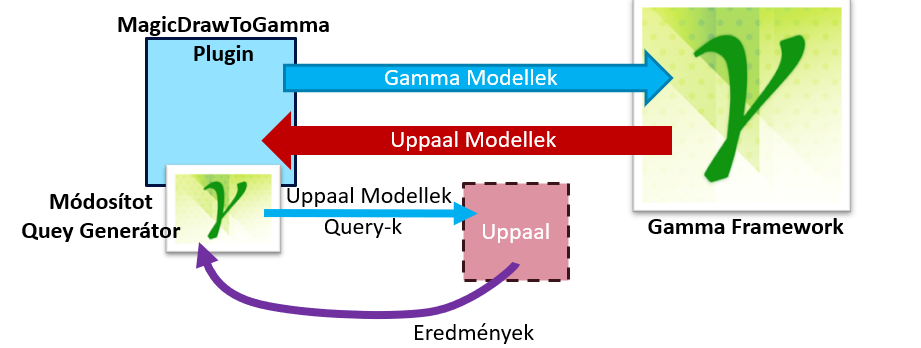
\includegraphics[width=100mm, keepaspectratio]{figures/concept.png}
	\caption{A plugin működése}
	\label{fig:concept}
\end{figure}

A plugin egyenlőre a back-annotationból származó információkat nem képes megjeleníteni, és csak single component állapottérképek transzformációjára képes.








\include{content/latex-tools}
\include{content/thesis-format}
\include{content/template-usage}


% Acknowledgements
%~~~~~~~~~~~~~~~~~~~~~~~~~~~~~~~~~~~~~~~~~~~~~~~~~~~~~~~~~~~~~~~~~~~~~~~~~~~~~~~~~~~~~~
%----------------------------------------------------------------------------
\chapter*{\koszonetnyilvanitas}\addcontentsline{toc}{chapter}{\koszonetnyilvanitas}
%----------------------------------------------------------------------------

Szeretnék köszönetet mondani mindazoknak a feladat elvégzése során segítették a munkám: Farkas Rebekának, aki konzulensemként mindig segítőkész, pozitív hozzáállásával, és szakmai tanácsival, kritikáival segítette a dolgozat létrejöttét. Továbbá Molnár Vincének aki a Gamma Statechart Composition Framework használatát javasolta és ötleteket adott a megvalósítható funkciókra vonatkozóan. Köszönöm továbbá az IncQuery Labs-nak, hogy rendelkezésemre bocsátották a plug-in skeletonjukat, és a náluk töltött szakmai gyakorlatom során szerzett gyakorlati tapasztalatokat, amik jelentősen megkönnyítették az implementáció elkészítését.


% List of Figures, Tables
%~~~~~~~~~~~~~~~~~~~~~~~~~~~~~~~~~~~~~~~~~~~~~~~~~~~~~~~~~~~~~~~~~~~~~~~~~~~~~~~~~~~~~~
%\listoffigures\addcontentsline{toc}{chapter}{\listfigurename}
%\listoftables\addcontentsline{toc}{chapter}{\listtablename}


% Bibliography
%~~~~~~~~~~~~~~~~~~~~~~~~~~~~~~~~~~~~~~~~~~~~~~~~~~~~~~~~~~~~~~~~~~~~~~~~~~~~~~~~~~~~~~
\addcontentsline{toc}{chapter}{\bibname}
\bibliography{bib/mybib}


% Appendix
%~~~~~~~~~~~~~~~~~~~~~~~~~~~~~~~~~~~~~~~~~~~~~~~~~~~~~~~~~~~~~~~~~~~~~~~~~~~~~~~~~~~~~~
%----------------------------------------------------------------------------
\appendix
%----------------------------------------------------------------------------
\chapter*{\fuggelek}\addcontentsline{toc}{chapter}{\fuggelek}
\setcounter{chapter}{\appendixnumber}
%\setcounter{equation}{0} % a fofejezet-szamlalo az angol ABC 6. betuje (F) lesz
\numberwithin{equation}{section}
\numberwithin{figure}{section}
\numberwithin{lstlisting}{section}
%\numberwithin{tabular}{section}

%----------------------------------------------------------------------------
%\section{A TeXstudio felülete}
%----------------------------------------------------------------------------
%\begin{figure}[!ht]
%\centering
%\includegraphics[width=150mm, keepaspectratio]{figures/TeXstudio.png}
%\caption{A TeXstudio \LaTeX-szerkesztő.} 
%\end{figure}


%\label{page:last}
\end{document}
